\chapter{Overview of Xen\label{cha:chapter3}}
This section provides background information on the Xen hypervisor and core components of its split device driver architecture for I/O emulation.

\section{Introduction of Xen\label{sec:xen}}
The Xen Project hypervisor is an open-source type-1 or baremetal hypervisor, which makes it possible to run many instances of an operating system or indeed different operating systems in parallel on a single machine (or host) \cite{xen}. It is one of the popular open-source hypervisors which can provide both para-virtualization and full virtualization solutions.In fact, it is the only available type-1 hypervisor which is open-source. It has been used in server and desktop virtualization and fueling the biggest clouds and web services in production today e.g. Amazon Web Services. 
\\
\\
Xen was developed at University of Cambridge in 2003 by Ian Pratt, a senior lecturer in the Computer Laboratory, and his PhD student Keir Fraser \cite{xen_wiki}. It was acquired by Citrix in 2007. Since April 15, 2013, Xen Project has become a Linux Foundation Collaborative Project with the following companies  contributing to and guiding the Xen Project as founding members are: Amazon Web Services, AMD, Bromium, Calxeda, CA Technologies, Cisco, Citrix, Google, Intel, Oracle, Samsung and Verizon \cite{xen_news}.
\\
\\
The basic components which work together to provide virtualization solution include Xen Hypervisor, Privileged guests called \textbf{Domain-0 or Dom0} and unprivileged guests called \textbf{Domain-U or DomU}. Xen hypervisor is a small software which directly runs on hardware and is responsible for CPU scheduling ,memory management and interrupt handling. After Xen hypervisor is booted, it launches Domain-0 guest which has direct access to all hardware and has native device drivers for performing I/O operations. Other unprivileged guests or domains access hardware and perform I/O via Dom0. Dom0 is also responsible for launching and managing DomUs with the help of control stack called Toolstack running on it. Figure \ref{xen_arch} shows the architecture of Xen virtual environment.
\begin{figure}[!htbp]
	\centering
	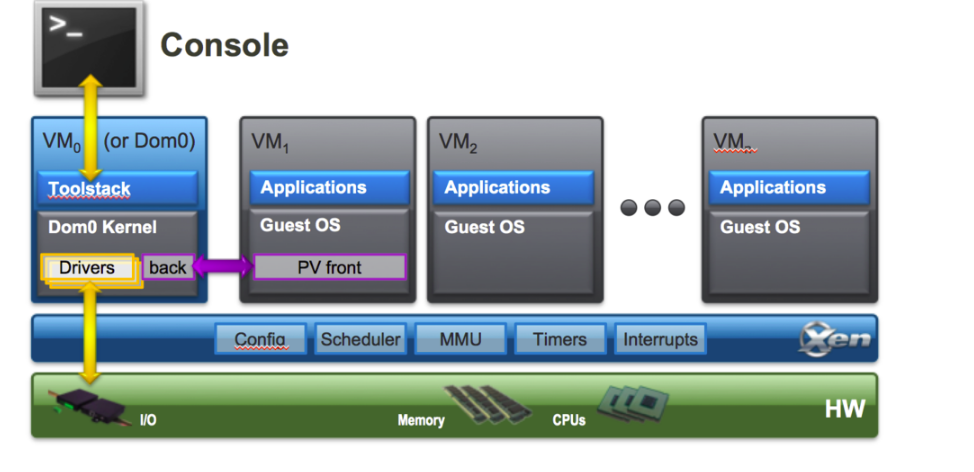
\includegraphics[width=10cm]{xen_arch}
	\caption{Xen Architecture Taken from \cite{xen_wiki}}
	\label{xen_arch}
\end{figure}
\\
\\
\subsection{Guest Virtualization Types in Xen \label{sec:guests}}
Xen provides two types of virtualization modes for guests:
\begin{itemize}
	\item  \textbf{Paravirtualization (PV)}, first introduced by Xen, is virtualization technique in which guests are modified and are aware of being run on a hypervisor. A PV guest requires PV enabled kernel and PV drivers to be present to run without emulation. Dom0 in Xen is a privileged PV guest which has access to actual device drivers and hardware in the system and provides an interface to control and manage other VMs.
	\item \textbf{ Hardware-assisted or Full Virtualization (HVM)} is a virtualization mode which requires virtualization hardware extensions (Intel VT or AMD-V hardware extensions) to be present on host CPU. Guests kernels are used unmodified and hence Windows can run as HVM guest on Xen.Xen uses Qemu on HVM guests for hardware emulation and hence are slower than PV guests. However, paravirtualized drivers can be used for I/O on HVM guests to increase performance of system.
\end{itemize}

Guests with both types of virtualization can be run at the same time on Xen. It is also possible to use paravirtualization on HVM guests and vice versa. This mixing of modes has introduced two more modes of virtualization on Xen which are PVHVM and PVH. In PVHVM guests, optimized paravirtualized drivers are used for disk and network virtualization on hosts with hardware virtualization extensions enabled. PVH are basically paravirtualized guests which use PV drivers for I/O operations and use hardware virtualization extensions for others.
\\
\\
There are pros and cons of each mode of virtualization in Xen. Full virtualization provides full emulation of underlying hardware to guests which require no modifications in their OSes. However, performance is degraded while providing full emulation of entire system by VMM. Also HVM guests use trap and emulate model for execution of sensitive and privileged instructions which can cost to hundreds to thousands of cycles \cite{wang2010dynamic}.. On the other hand, paravirtualization allows modified guests to run on a system with an abstraction of similar physical hardware on system and hence provides near native performance as compared to HVM guests. It replaces the sensitive instructions with hypercalls to VMM and allows combining several hypercalls into one hypercall to reduce transitions between Guests OS and VMM \cite{wang2010dynamic}.

\section{Device I/O Emulation on Xen\label{sec:xendevice}}
Xen hypervisor virtualizes CPU, memory, interrupts and timer. It does not have any knowledge of I/O devices. Access to actual physical I/O devices and their native device drivers is present in privileged Domain-0. Unprivileged guests can get access to I/O devices through Dom0. Xen assigns all I/O devices to Dom0 which is then responsible for MMIO remapping and interrupt handling. \\
\\
Device virtualization in Xen is done using a pair of paravirtualized drivers called \textbf{frontend and backend drivers}. For each class of hardware devices i.e. disk, network, console, framebuffer, mouse, keyboard, etc, a pair of paravirtualized drivers is present in system. Paravirtualized backends are implemented in Dom0 with their corresponding frontends being implemented in DomU. These paravirtualized drivers are implemented as kernel drivers. However, some backends can run in QEMU in userspace. Communication between frontends and backends is done through a shared memory ring protocol and events notifications mechanism provided by Xen. Xen provides tools to setup communication framework between frontend and backend drivers in Dom0 \cite{xen_arm}. Figure \ref{xen_device} shows the I/O device virtualization architecture in Xen.

\begin{figure}[!htbp]
	\centering
	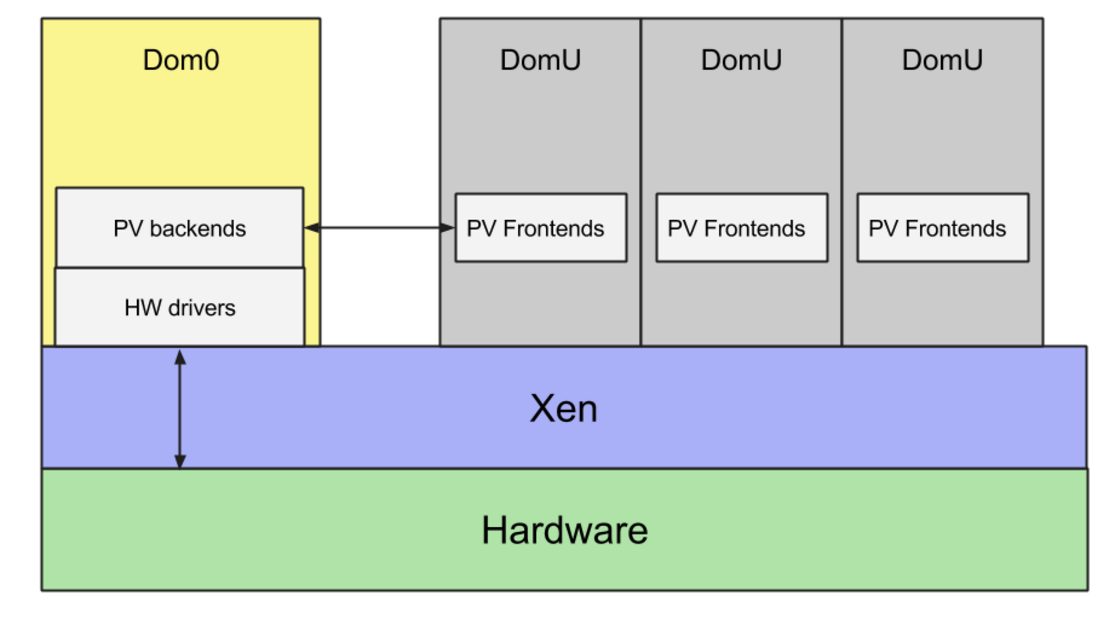
\includegraphics[width=10cm]{XEN_Device_Arch}
	\caption{Xen I/O Device Virtualization Architecture. Taken from \cite{xen_arm}}
	\label{XEN_Device_Arch}
\end{figure}

In order to provide isolation, security and disaggregation, Xen has introduced the concept of driver domains. Such domains are unprivileged guests running backends and native drivers for I/O device virtualization. If such a domain is compromised or crashed, it will not affect other guests or domains. Figure \ref{driver_domain} shows the architecture of driver domains in Xen.

\begin{figure}[!htbp]
	\centering
	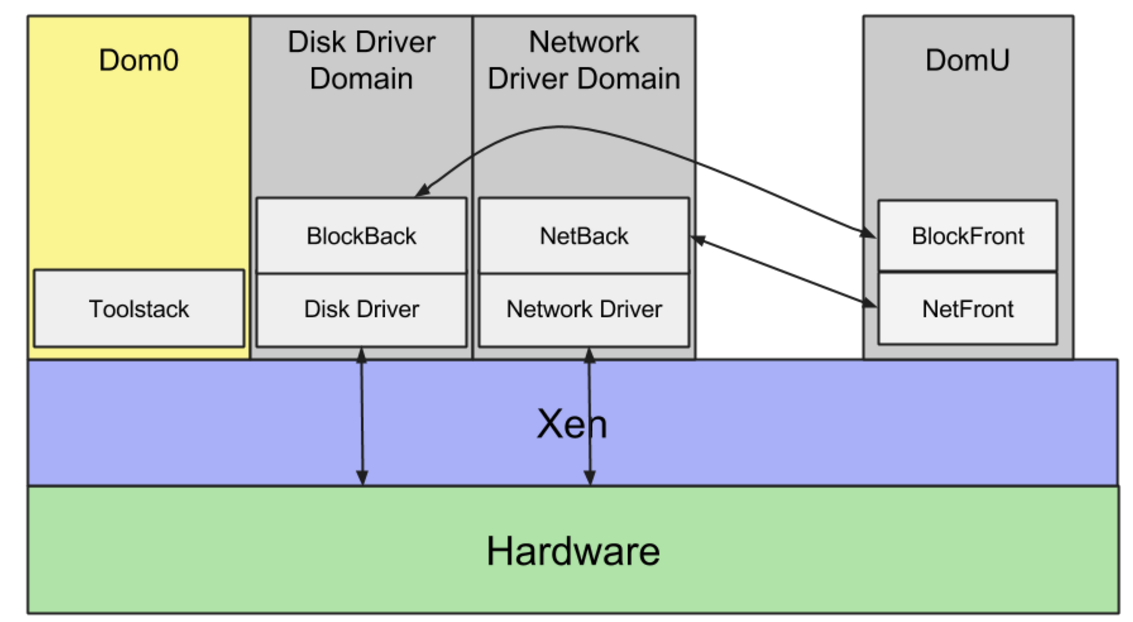
\includegraphics[width=10cm]{driver_domain}
	\caption{Xen Driver Domains Architecture. Taken from  \cite{xen_arm}}
	\label{driver_domain}
\end{figure}

\subsection{Xen on ARM\label{sec:xendevice}}
Xen on ARM is a simple, smaller and faster as compared to its x86 counterpart. The main features of Xen on ARM are described as follows:
\begin{itemize}
	\item It does not perform any emulation. There is no QEMU emulation in Xen on ARM.
	\item It exploits hardware virtualization support for memory management, interrupts and timer virtualization.
	\item It uses paravirtualized pair of drivers for I/O virtualization.
	\item It runs entirely in hypervisor mode and provides an HVV hypercall to kernels to switch between hypervisor mode and kernel mode.
	\item It uses virtualization aware Generic Interrupt Controller for interrupt handling.
	\item It uses virtualization aware Generic Timers to provide timer virtualization to guests.
	\item It supports one type of guests which exploits hardware virtualization as much as possible and uses paravirtualized interfaces for I/O device virtualization.
\end{itemize}

Figure \ref{xen_on_arm} shows the simple architecture for Xen on ARM platforms.
\begin{figure}[!htbp]
	\centering
	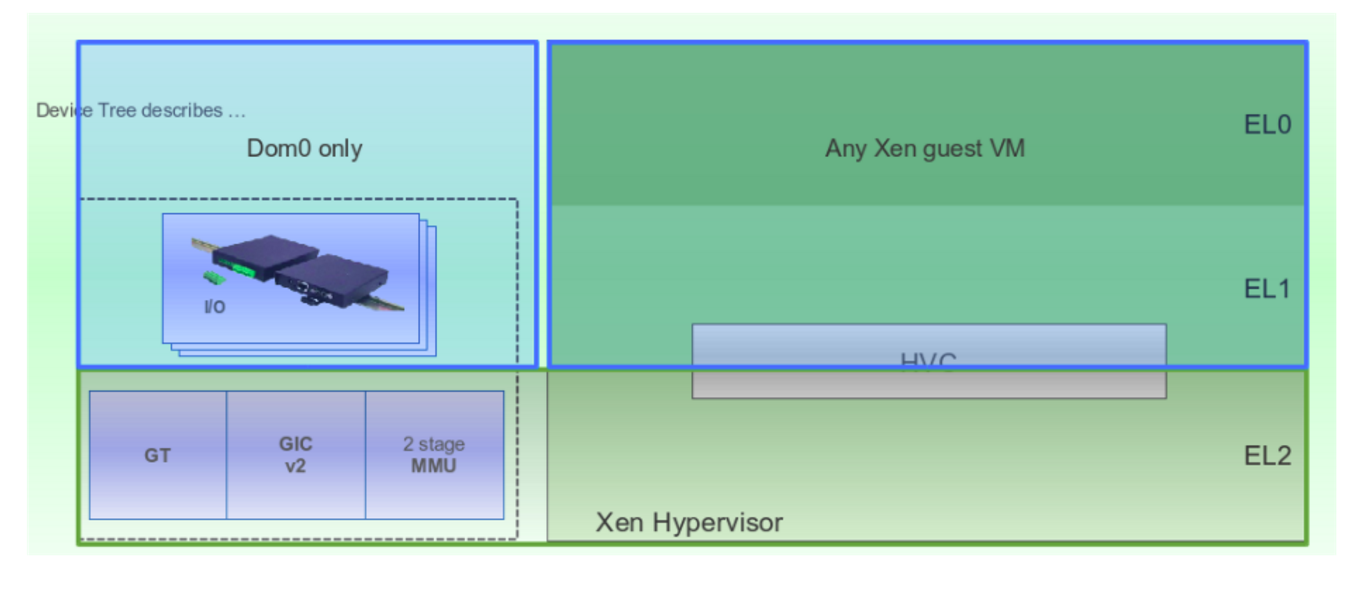
\includegraphics[width=10cm]{xen_on_arm}
	\caption{Xen on ARM Architecture. Taken from  \cite{xen_arm}}
	\label{xen_on_arm}
\end{figure}

\section{Xen Split I/O Driver Model\label{sec:xensplit}}
With the widespread use of embedded systems in multiple applications, diversity in I/O devices used by such systems has increased significantly. Supporting a large of I/O devices in Xen would make things worse for maintaining Xen hypervisor code and avoiding bugs. Most operating systems e.g Linux provide support for a large number of devices and reusing this capability would make a cleaner, smaller and much simpler hypervisor. Xen has delegated all I/O hardware devices to privileged Domain-0 or special unprivileged driver domains. All other guests access I/O devices through Dom0 or driver domains. Xen provides mechanisms for communication between guests which use split driver model for multiplexing and using hardware I/O devices. Xen support Net, Block, console, keyboard, mouse, framebuffer, XenGT(intel Graphic
card), 9pfs, PVCalls, Multi Touch, Sound and Display devices \cite{xen_release}. In the next sections, details of basic components of split driver model of Xen will be explained.

\subsection{Basic Components of Xen Split I/O Driver Model\label{sec:basiccomp}}
Xen device drivers typically consists of four major components:
\begin{itemize}
	\item The native I/O device driver
	\item Top half or Frontend of the split driver
	\item Bottom half or backend of the split driver
	\item Shared ring buffers
\end{itemize}

The real drivers for I/O devices are present in Dom0 or driver domains for accessing actual hardware. They are interfaced with backend drivers of the split driver which provides a generic interface and I/O device multiplexing functionality. Frontend driver is present in unprivileged guests and communicate with backends using shared memory ring buffers. Frontends write requests on these buffers and backends write responses which are signaled through xen event notification mechanism. Successful shared memory communication between frontend and backend requires xen grant tables, event channels, xen bus and Xenstore to be working in system. These mechanism will be explained in the later sections. Figure \ref{splitdevice} shows the basic architecture of Xen split driver mode.
\begin{figure}[!htbp]
	\centering
	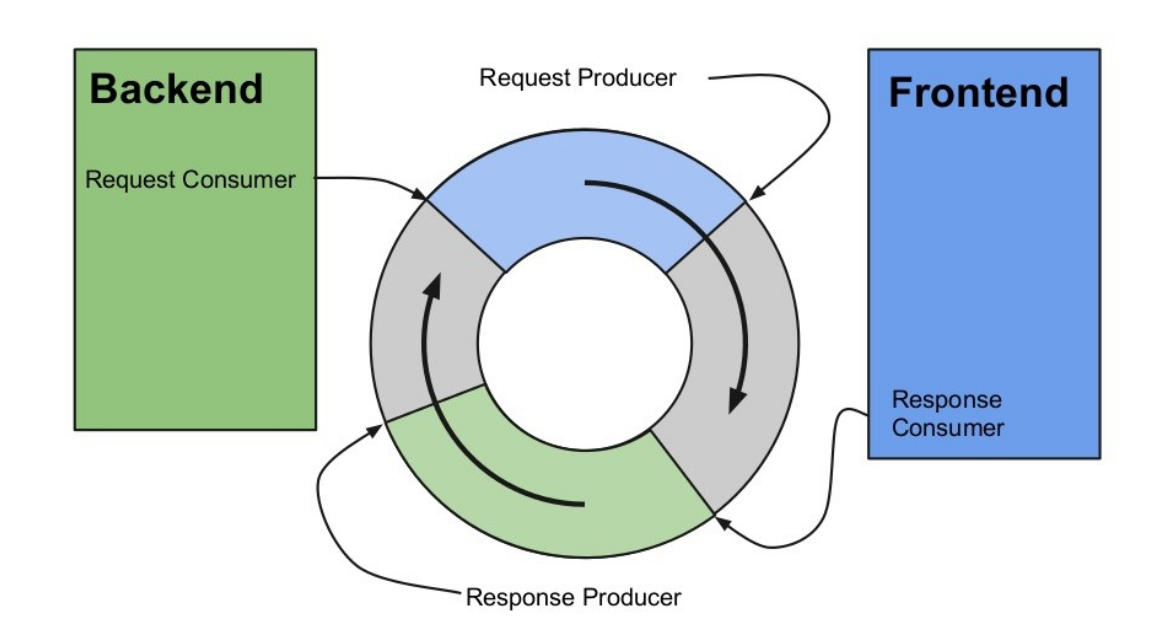
\includegraphics[width=10cm]{splitdevice}
	\caption{Basic Xen Split Driver Architecture. Taken from \cite{xen_slides}}
	\label{splitdevice}
\end{figure}

\subsection{Xen mechansims used by Split I/O Driver Model\label{sec:basicmech}}
There are basically four mechanisms provided by Xen which are used by Split Driver model of Xen to work successfully. These are as follows:
\begin{itemize}
	\item Grant Tables
	\item Event Channels
    \item Xenstore
	\item XenBus Protocol
\end{itemize}
The split drivers across domains use these mechanisms to communicate and access hardware devices. Following sections provide brief explanation of each of these mechanisms.
\subsubsection{Xen Grant Tables\label{sec:granttables}}
Grant tables is a mechanism to provide shared memory to guests. Each guests can manipulate the shared memory on page level granularity. Grant tables provides two types of memory sharing operations to guests i.e. memory sharing and memory transferring. Since all physical memory is mapped by Xen hypervisor, copying the data between domains is done by hypervisor without modifying page tables. Transferring a page from one domain to another is also available which changes the page owner and modifies the page tables accordingly. To identify the page being shared or transferred, guests uses grant references which are integers indexed into an array of grant entries in grant table. These grant references are placed in Xenstore ,a virtual file system for device discovery in Xen, to communicate shared page information to other domains.
\\
\\
The interface to grant tables is provides by Xen in the form of hypercalls for grant table operations. Two basic operations that can be performed on grant tables are mapping and transferring pages. Mapping a page removes original reference of page in sender domain's address space while transferring causes the page to leave calling domain's address space. Mapping is used by drivers to implement interdomain communication using shared memory while transferring is used to move data between domains. 
\\
\\
Xen hypervisor creates four types of structures to implement grant table mechanism:
\begin{itemize}
	\item Shared Grant table is created and shared by Xen for each guest. Guest writes into entries in table and Xen performs the desired operation specified by hypercalls. Four pages are allocated and shared with each guest during initialization of each domain. A maximum of 32 pages can be allocated for shared grant tables.
	\item Active Grant table is created and maintained by Xen to keep track of active grants per domain. Four pages are allocated initially for implementing active grant table per domain by Xen.
	\item Mapped track table is created and maintained by Xen per domain for each mapped page. Initially 1024 map track entries are allocated for each domain by Xen.
	\item Status Grant table is created and maintained by Xen for keeping track of status of each grant per domain.
\end{itemize}
Figure \ref{granttable} shows the basic structure of shared grant table.

\begin{figure}[!htbp]
	\centering
	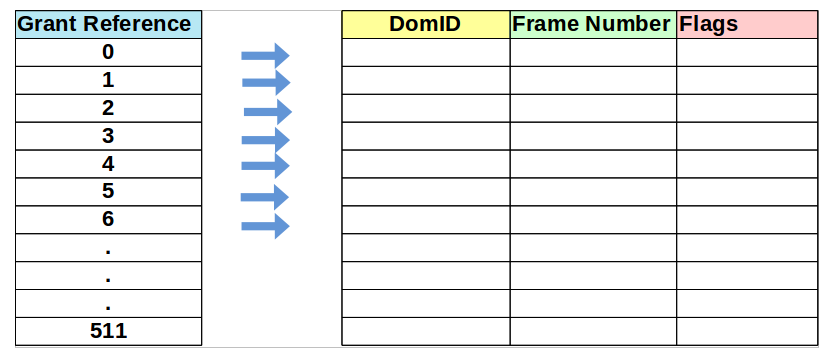
\includegraphics[width=10cm]{granttable}
	\caption{Basic structure of shared Grant table}
	\label{granttable}
\end{figure}
\textbf{Grant Table Use for Shared Ring Buffers}
Device I/O rings which are used for communication between split drivers are built on top of shared memory provided by grant table mechanism. Frontend drivers creates ring buffer pages and grant access to backend. Backend drivers map these shared pages for ring buffers and communication channel is established across domains. Figure \ref{ring} shows the actions performed by split drivers on ring buffers for interdomain communication.

\begin{figure}[!htbp]
	\centering
	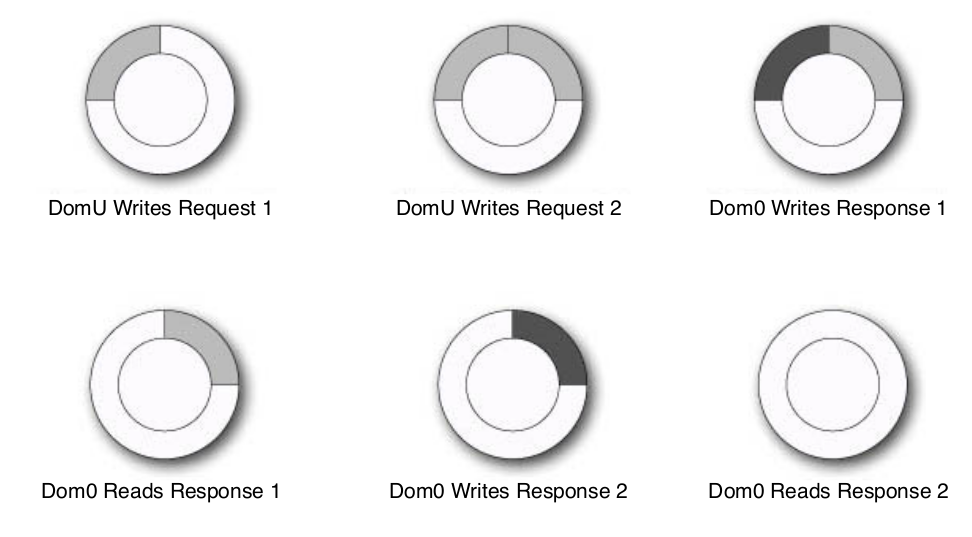
\includegraphics[width=10cm]{ring}
	\caption{Request/Response sequence on ring buffers. Taken from \cite{xen_book}}
	\label{ring}
\end{figure}
\subsubsection{Xen Event Channels\label{sec:eventchannel}}
Event channels is a mechanism for asynchronous delivery of notifications between domains. These are used with shared memory mechanism to provide message passing between split drivers in domains. Events are similar to Unix signals. Each event represents one bit of information about which event has occured. There are four types of event channels supported by Xen:
\begin{itemize}
	\item Interdomain events are used by split drivers for notifying each other about data waiting to be transported to other domain.  These are bi-directional.
	\item Physical IRQ are used to bind actual hardware IRQs to event channels. These are used by Domain-0 or driver domains to access various devices under their control by mapping physical IRQs to event channels.
	\item virtual IRQs (VIRQ) are used to bind IRQs of virtual devices e.g virtual timer or emergency console to event channels.
	\item Intradomain events are used to send events between virtual CPUs of a single domain similar to interprocessor interrupt (IPI) mechanism. These are bi-directional.
\end{itemize}

Event channel creation is a two-stage process. In the first step, an event source is bound to event channel and in second step, an event handler is registered for handling triggered event. Event channel is an abstraction of sending asynchronous notifications between domains. Each channel has two endpoints which are called ports in local domain. After binding an event channel to remote port, a domain can send an event to local port via hypercall through Xen hypervisor. Xen is then responsible for finding the remote end of channel and remote domain and route events to destination.
\\
\\
Each virtual CPU in the guest on Xen has an event channel bitmap associated with it. This event channel bitmap is shared with Xen in shared info page created during initialization of guest. When an event is received by Xen for a particular guest, it sets event channel upcall pending flag, desired bit of event and corresponding word which contains set event bit. All these fields are present in shared info page. There are also mask bits for disabling event delivery to guests. Events delivery can be masked both by individual event type or disabling/enabling all together.
\\
\\
Two implementations of event channels are supported in Xen \cite{xen_events}:
\begin{itemize}
	\item 2-level event channel ABI is de-factor implementation for event channel mechanism for which 32 bit domain supports up to 1024 event channels and 64 bit domain supports up to 4096 channels.A 2-level search path is used for finding the set event bit in event channel bitmap. For the thesis, 2-level event channel has used since it meets the requirements for porting I/O split driver to PHIDIAS.
	\item FIFO-based event channel ABI has lockless queues for event queues with configurable number of event channels and event priorities. It can support more thanm 100,000 event channels, with scope for  16 different event priorities.
\end{itemize}
Figure \ref{events_slide} shows the basic architecture of 2-level event channel implementation.

\begin{figure}[!htbp]
	\centering
	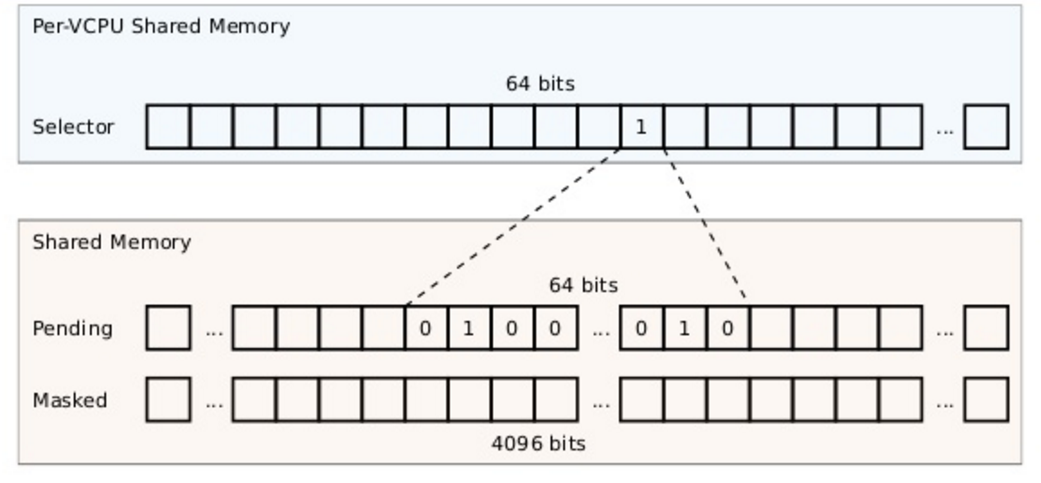
\includegraphics[width=10cm]{events_slide}
	\caption{2-level event channel implementation in Xen. Taken from \cite{events_slide}}
	\label{events_slide}
\end{figure}
\subsubsection{Xenstore \label{sec:xenstore}}

